\documentclass[11pt]{article}

\usepackage{graphicx}
\graphicspath{{../results/}}


%% Useful packages
\usepackage{amsmath,amssymb}
\usepackage{graphicx}
\bibliographystyle{unsrt}
\usepackage{tabularx}
\usepackage{kantlipsum}
\usepackage{booktabs}
\usepackage[normalem]{ulem}
\useunder{\uline}{\ul}{}
\usepackage{amsmath}
\usepackage{lineno}
\usepackage{biblatex} 
\addbibresource{Report.bib}
\usepackage[round]{natbib}

\graphicspath{{../results/}}

\linenumbers



\begin{document}

\title{Non-linear models outperform linear models in predicting bacterial growth}

\author{Uva Fung}

\date{Word count: 3131}


\begin{abstract}
Predicting bacterial growth is important in the food industry as the information can be used to determine food shelf life. Bacterial growth can be modelled using different approaches, which would influence the accuracy of the prediction. Here, I compared six models to identify the best one to be used in predicting bacterial growth. I also investigated if the use of multiple starting parameter values improved model fitting. This study show that non-linear models perform better than linear models. Gompertz model with multiple starting parameters have the highest number of converged datasets. Taking into account the significance of fitting, the Baranyi model is the best fitting one once the model successfully converges. 
\end{abstract} 


\section{Introduction}
The study of bacterial growth is important in food microbiology as it provides important information in determining shelf life and food safety \citep{zwietering_modeling_1990}. The growth of bacteria over time can be separated into four phases: lag phase, exponential growth phase, stationary phase and dead phase \cite{wang_bacterial_2015}, which can be modelled using different phenomenological and mechanistic approaches \cite{johnson_model_2004, peleg_microbial_2011}. Some simple phenomenological models only include time as the explanatory variable in predicting population growth. These models can be fitted quickly within a short period of time but with limited fitting accuracy. Other more complex ones, such as the Gompertz model, incorporates specific growth rate to improve goodness of fit. However, all phenomenological models only describe the pattern of bacterial growth and do not provide explanations on what causes the observed pattern \cite{peleg_microbial_2011}. Mechanistic models take into account additional biological parameters, such as growth rate, length of lag phase, initial and final population sizes, providing biological explanations on the observed patterns \cite{zwietering_modeling_1990}.The starting values for parameters can be further searched for and adjusted during model fitting to obtain the optimal model. Some of the most popular mechanistic models include the Logistic model \cite{zwietering_modeling_1990} and the Baranyi model \cite{baranyi_dynamic_1994}. These models generally provide a better fit, but take a longer processing time and might not converge well depending on the starting parameters. The use of different models could have drastic differences in the predicted bacterial growth. This in turn could have a huge effect on the food industry, as models that predict bacterial growth poorly could cause wrong estimations of shelf life, leading to food wastage or hygiene and public health issues. 
\vspace{\baselineskip}

This study aims to identify the best model to be used in predicting bacterial growth across large empirical datasets. I will answer four questions: i) Which model has the highest number of successfully converged datasets? ii) Which model has the highest number of best fit across all datasets? ii) What is the time needed to fit each model? iv) Does the search for multiple starting parameter values increase the number of successful fitting in Gompertz and Baranyi models? I hypothesized phenomenological models to spend a much shorter fitting time than mechanistic models because the latter has multiple biological parameters. I also expect the search for starting parameter values should increase the number of successful model fits in both Gompertz and Baranyi models, as this should increase the likelihood of sampling a starting parameter close enough for convergence. The best model will be determined based on the number of datasets successfully converged, the number of datasets that are best fitted by the model, and the time needed to complete the model fitting process.



\section{Methods}

\underline{Data collection} 

A total of 305 experimental datasets measuring bacterial growth over time were extracted from ten peer-reviewed published papers \cite{roth_continuity_1962, stannard_temperaturegrowth_1985, phillips_relation_1987, sivonen_effects_1990, zwietering_modeling_1990, gill_growth_1991, bae_growth_2014, galarz_predicting_2016, bernhardt_metabolic_2018, silva_modelling_2018}. Each dataset recorded change in bacterial population size at different time points. These datasets consist of a combination of 45 different bacteria species grown in 18 different mediums at 17 different temperatures. A large range of species, mediums and temperatures were chosen in order to test that each model can be fitted to bacterial growth in different experimental settings. 
\vspace{\baselineskip}

\underline{Data wrangling}

Data wrangling and analysis were done in R (ver 3.6.3). Data was first filtered to remove data points with population size and time smaller than zero, as these represents incorrect measurements or error in data input. Datasets with fewer than 6 time points were also removed as the number of data points is too low for good quality model fitting. 
\vspace{\baselineskip}

\underline{Model fitting} 

For each dataset, I fitted six models: four phenomenological models (Ordinary Least Squares (OLS), Quadratic equation, Cubic equation, Gompertz model) and two mechanistic models (Logistics model, Baranyi model). Three models are fitted using the linear regression approach (OLS, Quadratic, Cubic). The remaining three (Logistic, Gompertz, Baranyi) are fitted using the non-linear least-squares (NLLS) approach, with parameters adjusted for using the Levenberg-Marquardt algorithm. The three non-linear models are chosen on the basis that they are the most popular models to be used in predicting bacterial growth. The logistic model is chosen as it can model complicated fluctuation patterns and chaos from a relatively a “simple” nonlinear process, while the Gompertz model is used across multiple disciplines and can describe growth curves having a long or short lag time \cite{zwietering_modeling_1990}. The Baranyi model is applicable under dynamic conditions with good fitting capacities \cite{poschet_analysis_2005}. The equations used are listed below.Notations in equations are as below: Time (\(t\)), Population size at time t (\(N_{t}\)), Population size at time 0 (\(N_{0}\)), population size at maximum (\(K\)), coefficients (\(m\), \(a\), \(b\), \(c\), \(d\)), maximum specific growth rate (\(r\)), time when lag phase ends (\(t_{lag}\)).


\begin{equation} 
  OLS: log \(N_{t}\) = \(m\)\(t\) + \(c\) 
\end{equation}

\begin{equation}
  Quadratic: log \(N_{t}\) = \(a\) + \(b\)\(t\) + \(c\)\(t^{2}\) 
\end{equation}

\begin{equation}
  Cubic: log \(N_{t}\) = \(a\) + \(b\)\(t\) + \(c\)\(t^{2}\) + \(d\)\(t^{3}\) 
\end{equation}

\begin{equation}
  Logistic: \(N_{t}\) = \frac{\(N_{0}\)K_{e}^{rt}}{K + N0(e^{rt}-1)} 
\end{equation}

\begin{equation} 
  Gompertz: log\(N_{t}\) = log(\(N_{0}\)) + (log(K) - log(\(N_{0}\))e^{-e*(r*e(1)*\frac{t_{lag} - t}{log(K) - log(\(N_{0}\))*log{10}}}+1 
\end{equation}

\begin{equation} 
  Baranyi: log(N_{t}) = N_{0}+r*A*N_{t}*t -ln(1 + \frac{e^{r*N_{0}*t}-1}{e^{(K - N_{0})}} 
\end{equation}

\begin{equation} 
  Baranyi: N_{t} = t - \frac{1}{r}*ln*(e^{-r*t}+e^{-r*t_{lag}}- e^{-r(t+t_{lag})}) 
\end{equation}


Each dataset consists of data to fit the three parameters (\(t\), \(N0\), \(K\)) using the graphical method \cite{holmstrom_review_2002}. Maximum specific growth rate (\(r\)) was obtained from the slope estimate of the Ordinary Least Squares linear regression output. The time point of \(t_{lag}\) was determined as the time point prior to the greatest population increase within the first half of the experimental duration. In order to increase the likelihood of successful model fitting for Gompertz and Baranyi models, I further fitted both models with the addition of searching for multiple starting values for \(t_{lag}\). The upper and lower ranges of \(t_{lag}\) was set as the first half of the experimental duration. staring parameters This allowed the model to search for multiple starting values and iterates through them to determine the best fitting model. The fitted values, standard residuals and Akaike Information Criterion (AIC) scores were calculated for each model fitting.
\vspace{\baselineskip}

\underline{Check for assumptions} 

After model fitting, I checked each model to see that the model fitted met the assumptions of homogeneity of variance and normality. For each model and dataset combination, I constructed residual vs fitted plots and Normal Q-Q plots. Datasets that did not fit the assumptions were removed from the analysis. A total of 284 datasets remained for subsequent model comparison.
\vspace{\baselineskip}

\underline{Model analysis}

I first compared the number of successfully converged datasets for each of the five fitted mechanistic models. I then compared the AIC scores across all eight models to determine which model has the lowest AIC score for each dataset. AIC are relative scores used for comparison between models. If two models have a difference in AIC scores of 2 or more, then the model with a lower AIC score fits significantly better (Akaike, 1974). Thus in each dataset, the model that is significantly the best fitting one was also identified. The time taken for running each model fitting function was then tested. 
\vspace{\baselineskip}

\underline{Computing tools}

Data wrangling, model fitting, assumption checking, model analysis and plotting were all done in R ver 3.6.3. Data wrangling was done using the \emph{tidyverse} package. Model fitting was done using \emph{broom}, \emph{stats}, \emph{minpack.lm} and \emph{nls.multstart} packages. Model fitting of OLS, quadratic and cubic equations was done using the \emph{lm()} function in the stats package. Logistic, Gompertz and Baranyi models were fitted using the \emph{nlsLM()} function in \emph{minpack.lm} package, which uses the Leven-Marquardt algorithm to search for the best fitting model. Gompertz and Baranyi models with multiple starting parameters were fitted using \emph{nls\textunderscore multstart()} function in \emph{nls.multstart} package. Run time for each function were tested using \emph{system.time()} function. Graph plotting was done using \emph{ggplot2} and \emph{ggforce} packages. 
\vspace{\baselineskip}



\section{Results}

Among the five fitted non-linear models, the logistic model has the highest number of successfully converged datasets and is fitted in 99.2\% of the datasets (Table 1). Both Gompertz and Gompertz with multiple starting parameter values (Gompertz msp) successfully fitted a similar percentage of datasets, with 55.6\% and 64.7\% successful convergence respectively (Table 1). The Baranyi model fitted the fewest number of datasets. Only 31.6\% and 28.1\% of datasets successfully converged using the Baranyi model and the Baranyi model with multiple starting values (Baranyi msp).
\vspace{\baselineskip}

\begin{table}[]
\caption{Number of datasets successfully converged by each non-linear model. NA refers to datasets that produce errors when fitted in the equation. Total number of datasets \(n\) = 284.}
\begin{tabular}{@{}lllll@{}}
\toprule
Models       & No. successful datasets & No. failed datasets & NA  &  \\ \midrule
Logistic     & 282                     & 1                   & 1   &  \\
Gompertz     & 158                     & 98                  & 28  &  \\
Baranyi      & 90                      & 4                   & 190 &  \\
Gompertz msp & 184                     & 35                  & 149 &  \\
Baranyi msp  & 80                      & 8                   & 196 &  \\ \bottomrule
\end{tabular}
\end{table}



Among the eight models fitted, Gompertz msp model is best fitted to the greatest number of datasets based on lowest AIC scores (78) followed by the Baranyi model (71) (Table 2). The OLS model has the fewest number of best-fitting datasets. Only 2.4\% of the total dataset returned the OLS model as the one with the lowest AIC. The use of multiple starting parameter values increases the number of datasets best fitted in the Gompertz msp model, but not in the Baranyi msp model (Table 2).
\vspace{\baselineskip}

Once the significance in AIC scores is taken into account, I found that out of the total 284 datasets, 135 datasets were equally best fitted by more than one model (two or more models with an AIC score difference <2) (Table 2; Fig. 1, Fig. 2). The remaining 149 datasets are significantly best fitted by a single model (Table 2; Fig. 3). Baranyi has the highest number of significantly best fitted datasets. When incorporating the number of successfully converged models, I found that the majority of the datasets successfully fitted by the Baranyi model return the Baranyi model as the one with the lowest AIC that fits significantly better than other models (Table 4). In contrast, only 5-8\% of the datasets successfully fitted by the Logistic, Gompertz, Gompertz msp or Baranyi msp models returned these four models as the ones with significant best fit.
\vspace{\baselineskip}

\begin{table}[]
\caption{Number of datasets best fitted by each model based on lowest AIC scores. Total number of datasets \(n\) = 284.}
\begin{tabular}{@{}lllll@{}}
\toprule
Model        & No. datasets with lowest AIC & No. significantly best fitted datasets &  &  \\ \midrule
OLS          & 5                            & 0                                      &  &  \\
Quadratic    & 14                           & 3                                      &  &  \\
Cubic        & 33                           & 20                                     &  &  \\
Logistic     & 52                           & 25                                     &  &  \\
Gompertz     & 15                           & 12                                     &  &  \\ 
Baranyi      & 73                           & 73                                     &  &  \\
Gompertz msp & 85                           & 12                                     &  &  \\
Baranyi msp  & 7                            & 4                                      &  & 
\end{tabular}
\end{table}

\vspace{\baselineskip}

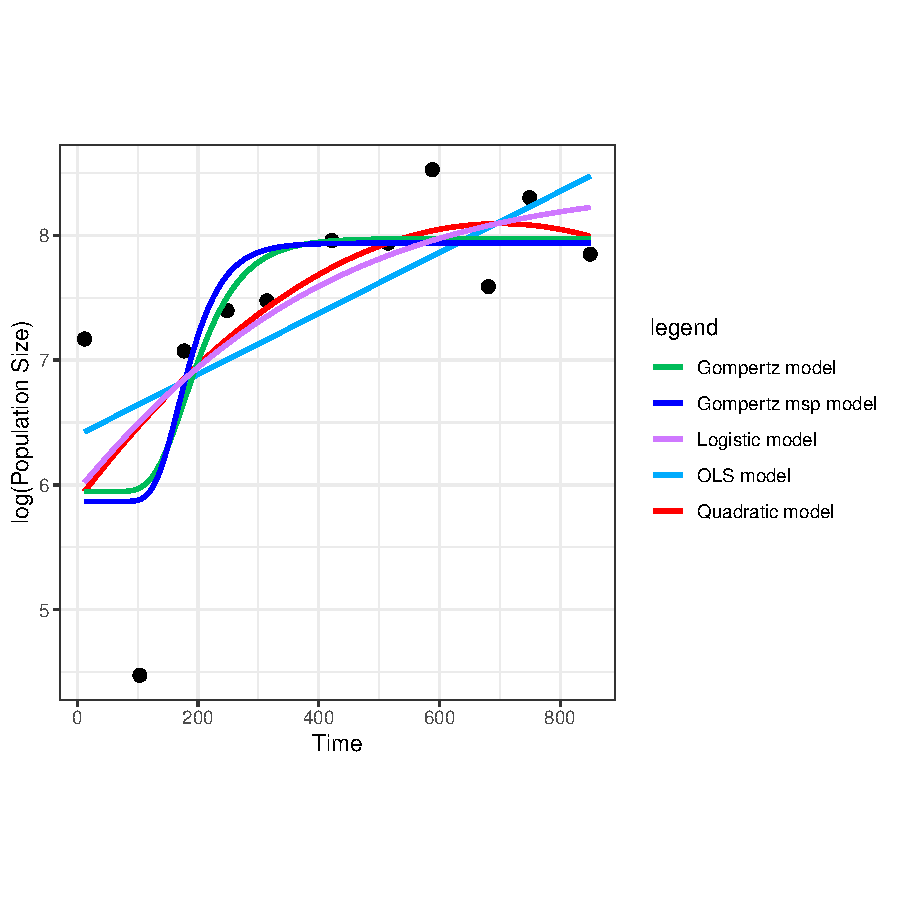
\includegraphics[width=0.5\textwidth]{../results/ID277.pdf}


{\footnotesize Fig 1: Model fitting in dataset ID277\textunderscore 1. All the models fitted do not differ significantly from each other and show a poor fit. }

\vspace{\baselineskip}

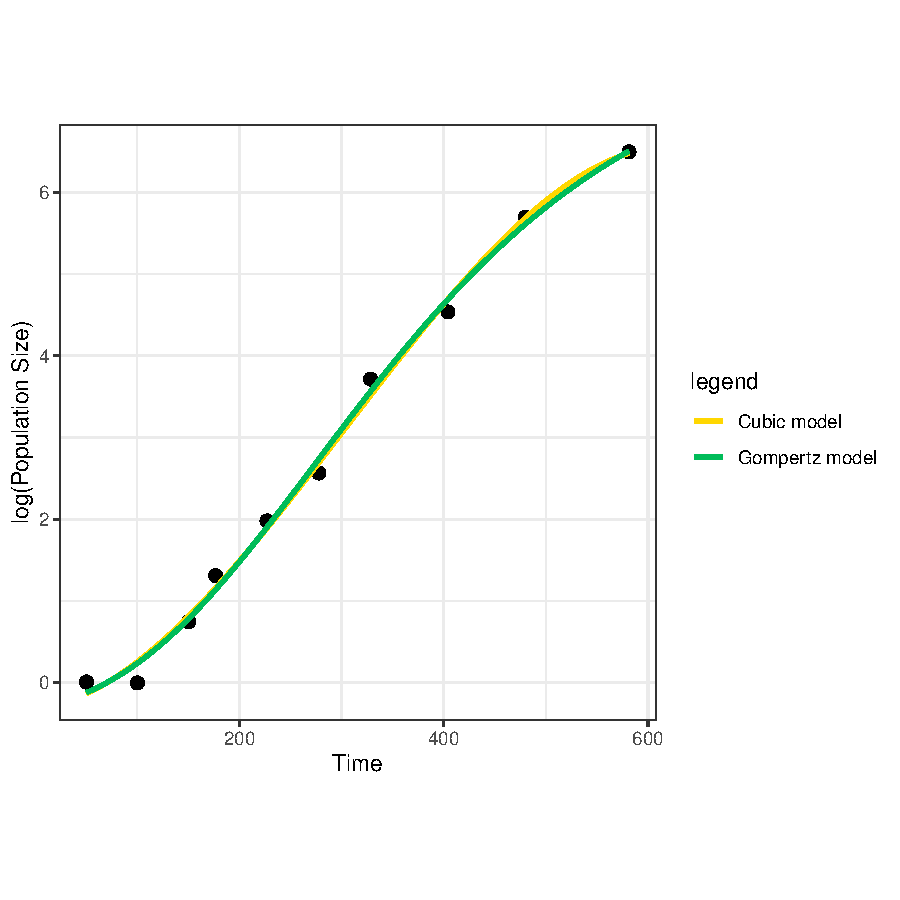
\includegraphics[width=0.5\textwidth]{../results/ID259.pdf}


{\footnotesize Fig 2: Model fitting in dataset ID259\textunderscore 1. Both Cubic and Gompertz are equally the best fitting models.  }

\vspace{\baselineskip}

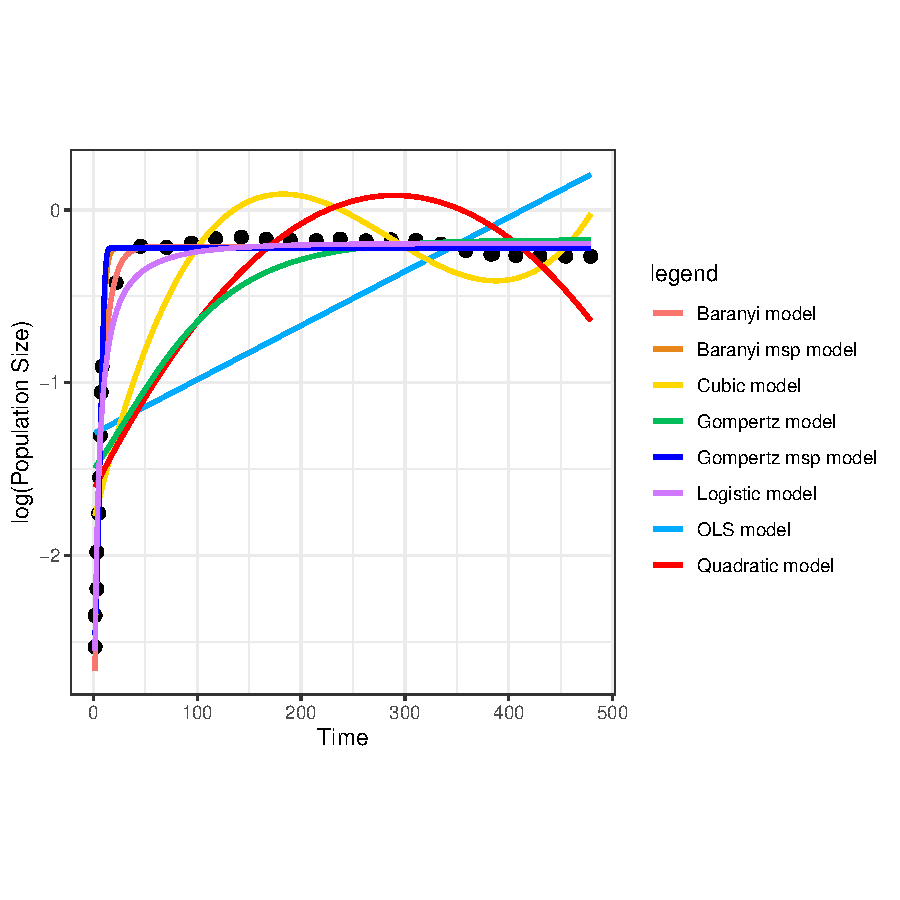
\includegraphics[width=0.5\textwidth]{../results/ID131.pdf}


{\footnotesize Fig 3: Model fitting in dataset ID131\textunderscore 1. The Baranyi model is significantly the best fitted model. }

\vspace{\baselineskip}

\begin{table}[h]
\caption{Percentage of significantly best fitted datasets relative to the total number of successfully converged datasets.}
\resizebox{\textwidth}{!}{%
\begin{tabular}{@{}lllll@{}}
\toprule
Model        & No. datasets converged successfully & No. datasets significantly best fitted & \% (No. significantly best-fitted datasets / No. successfully converged datasets) &  \\ \midrule
Logistic     & 282                                 & 25                                     & 8.86\%                                                                            &  \\
Gompertz     & 158                                 & 12                                     & 7.59\%                                                                            &  \\
Baranyi      & 90                                  & 73                                     & 81.1\%                                                                            &  \\
Gompertz msp & 184                                 & 12                                     & 6.52\%                                                                            &  \\
Baranyi msp  & 80                                  & 4                                      & 5\%                                                                               &  \\ \midrule
             &                                     &                                        &                                                                                   &  \\
             &                                     &                                        &                                                                                   &  \\
             &                                     &                                        &                                                                                   & 
\end{tabular}}
\end{table}


All three linear models (OLS, Quadratic, Cubic) have a similar user run time between 0.009 - 0.013s per dataset. The run time for non-linear models is relatively longer (table 4). Among them, the logistic model takes the shortest time to run (0.021s), followed by Baranyi and the Gompertz model. The addition of multiple starting parameter values greatly increases the run time of Gompertz and Baranyi models to 3.057s and 7.692s respectively. 

\vspace{\baselineskip}

\begin{table}[]
\caption{Time (in second) taken to fit each model and generate AIC outputs.}
\begin{tabular}{@{}lllll@{}}
\toprule
Model        & User  & System & Elapsed &  \\ \midrule
OLS          & 0.013 & 0.001  & 0.015   &  \\
Quadratic    & 0.012 & 0.001  & 0.017   &  \\
Cubic        & 0.009 & 0.001  & 0.010   &  \\
Logistic     & 0.021 & 0.006  & 0.028   &  \\
Gompertz     & 0.113 & 0.034  & 0.155   &  \\
Baranyi      & 0.040 & 0.009  & 0.052   &  \\
Gompertz msp & 3.057 & 0.874  & 5.667   &  \\
Baranyi msp  & 7.692 & 1.861  & 13.285  & 
\end{tabular}
\end{table}



\section{Discussion}
This study aims to identify the best model in modelling bacterial growth across datasets, determined based on the number of successful convergence, the number of best fitted datasets and the time needed to fit the model. Among all non-linear models, the Logistic model has the highest percentage of successful convergence (99.2\% of datasets), and the lowest percentage in the Baranyi msp model. One reason is that the Baranyi model has a more complex equation involving a logarithm term ln (e- + e- -ee). If the dataset produces a negative value, then the logarithmic function would not work and an error message would return \cite{wiscombe_exponential-sum_1977}. For example, a small growth rate, short lag period, and a long total time would lead to a negative value, in which taking its logarithmic term would return an error and the model cannot be fitted. Another reason is because the Baranyi model uses an additional parameter (\(t_{lag}\)). The non-least square method works by searching for a combination of parameter values that is closest to the optimal least-squares solution with the smallest sum of squared residuals possible \cite{see_parameter_2018}. If the starting \(t_{lag}\) value is poorly estimated and too far off from the optimal value, then the model would fail to identify the optimal least-squares solution and cannot converge. This could be the case in this study as both Gompertz and Baranyi models incorporate an extra tlag parameter, while the Logistic model does not have this parameter.  
\vspace{\baselineskip}

Based on the lowest AIC scores, the Gompertz msp model gave the highest number of best fitted datasets followed by the Baranyi model. The linear models are generally poorly fitted than the non-linear ones because the former does not take into account biological parameters (such as specific growth rate or lag phase), whereas these are included in the non-linear models \cite{peleg_microbial_2011}. Another reason is that the linear model fits the data points directly using linear regression, whereas the non-linear models are fitted using non-linear least squares, which would adjust parameter values to search for the best model. As a result, there is a higher chance for the best-fitted model to be identified using non-linear approaches. 
\vspace{\baselineskip}

However, when taking the relative difference in AIC scores between models into account, Baranyi model was the only model that is significantly better than all other models. All 73 datasets best fitted by the Baranyi model fit significantly better than other models based on a difference in AIC scores of 2 or more. For example, the Baranyi model is the best fitting one of all eight models in dataset 131\textunderscore 1 (Fig. 3), as only the Baranyi model line passes through all data points. In contrast, the Gompertz msp model, which has the lowest AIC score in 85 datasets, only significantly best fits 12 datasets. One explanation is because the data fitted are of poor quality and did not show a distinctive lag, growth and stationary phase. For example, the data points in dataset 227\textunderscore 1 (Fig. 1) are scattered and lack a clear growth phase. Thus in this dataset, none of the five fitted models (Gompertz, Gompertz msp, Logistic, OLS or Quadratic model) fits the data significantly better than others. Another possibility is that the data only captures part of the bacterial growth, such that it is also a good fit when implementing other models. An example is dataset 259\textunderscore 1 (Fig. 2), which only records the growth phase of the bacteria. The resultant isothermal curves can be fitted by both cubic and the Gompertz model \cite{peleg_microbial_2011}, and therefore both models best fit this dataset. It is also worth noting that in the Baranyi model, 81.1\% of the successfully converged datasets return Baranyi model as the best fitting one. This implies that once successfully converged, the Baranyi model generally is the best fitting model. 
\vspace{\baselineskip}

In line with my hypothesis, The use of non-linear least-square methods and multiple starting parameter values both increase the time needed to run the model. Unlike linear models which directly fit the parameters in the equation, extra time is needed in NLLS to adjust the parameters to search for the best combination of parameters \cite{kallehauge_comparison_2016}. The inclusion of multiple starting parameters further increases the time needed, as additional time is needed to search for the best starting \(t_{lag}\) values. In particular, the Baranyi msp model takes more than twice the time to run than the Gompertz msp model. This is because the Baranyi has a more complex equation and therefore would take longer to compute. 
\vspace{\baselineskip}

The long time spent in Gompertz msp is compensated by the higher number of successful convergence and the greater number of datasets fitted with the lowest AIC scores. However, after taking into account the significance of AIC between models, both Gompertz and Gompertz msp significantly fitted 12 datasets only. This suggests that the inclusion of multiple starting parameter values in the Gompertz model did not improve model fitting. This could be because the initial starting parameter value based on graphical methods was not optimal \cite{holmstrom_review_2002}, or that the Levenberg–Marquardt algorithm used in searching for the optimal model has limited searching ability and fail to identify more optimal parameter values for model fitting \cite{transtrum_improvements_2012}. The former can be improved by estimating using the geometrical sums method, which involves generalized interpolations \cite{holmstrom_review_2002}. The latter is a common constraint in models with multiple parameters known as parameter evaporation \cite{transtrum_why_2010}. In the Gompertz msp model, it is possible that only a few parameter combinations are relevant to finding the optimal model, whereas most other combinations do not return a better fit. Therefore during model fitting, the Levenberg–Marquardt search algorithm might got lost in regions of parameter space. The algorithm would then push the parameters to infinite values without finding a good fit. Similarily, the fewer number of successfully converged and best fitted datasets in the Baranyi msp model could also be attributed to parameter evaporation. It is suggested that the Leven-Marquardt search can be improved by including corrections in the approximation of residuals \cite{transtrum_improvements_2012}. Other search algorithms using hybrid Gauss–Newton (GN) and quasi-Newton algorithms are recommended \cite{holmstrom_review_2002}. The use of Maximum Likelihood and Bayesian approaches in choosing parameter searching for optimal model could also improve model fitting, especially in datasets with small sample sizes \cite{zondervan-zwijnenburg_pushing_2018}. 
\vspace{\baselineskip}

To conclude, Gompertz model has the highest number of successful convergence and best fit based on lowest AIC. However, taking into account the significance of AIC scores, the Baranyi model is the best at fitting across multiple datasets once successfully converged. Evidence from this study does not support the use of multiple starting parameter values in Gompertz or Baranyi models, due to the long run time and the lack of improvement in data fitting. Future studies could focus on including multiple starting values for more parameters (eg. specific growth rate), optimizing the search method for starting parameter values, and adopt more advance search algorithms. Improvements in code vectorization could reduce the run time needed for models fitted with non-linear least-square methods. 
\vspace{\baselineskip}





\bibliographystyle{plainnat}
\bibliography{Report.bib}

\printbibliography

\end{document}